\section{Proposed Approach and System Overview}\label{sec:architecture}

This section bridges the requirements of Section~I to the detailed technical parts that follow. We first present the hybrid DT/PT architecture (Contribution 1) that is designed offline and realized at deployment/operation time. We then explain the evaluation principle (Design-Space Exploration) that motivates our empirical validation campaign (Contribution 2).

\subsection{Evaluation Principle: Design-Space Exploration (DSE) for Architectural Validation}\label{subsec:design_space}

A dedicated evaluation environment (simulation/emulation) enables the designer to:
\begin{itemize}
    \item \textbf{Explore architectural alternatives:} Vary the structure, size, and perception range of mobile assets or agents to study their impact on system-level properties letated to missions.
    \item \textbf{Experiment with control algorithms and parameters:} Test different local rules, coordination mechanisms, and behavioral parameters to assess their influence on emergent behaviors.
    \item \textbf{Analyze results across multiple metrics:} Quantitatively evaluate each candidate design using metrics such as coverage, resilience, scalability, efficiency, and responsiveness.
\end{itemize}

\noindent The DSE campaign systematically explores the relationships between \textbf{fleet constitution} (number of drones, initial spacing, spare availability), \textbf{hazard scenarios} (single loss, cascading failures, adversarial intrusions), and \textbf{mission outcomes} (coverage maintenance, recovery time). This parametric exploration produces dimensioning guidance: given expected hazard frequencies and required resilience levels, what fleet size and spare inventory suffice to maintain acceptable coverage?

Full experimental protocols, scenario definitions, and simulation implementation details are presented in Section~\ref{sec:methodology}. This section focuses on the architectural design that emerges from DSE findings.

\subsection{Decision Support from Evaluation Outputs}

Simulation outputs are systematically analyzed to:
\begin{itemize}
    \item \textbf{Identify trade-offs and Pareto-optimal solutions:} Balance competing objectives and constraints based on stakeholder priorities and mission context.
    \item \textbf{Support data-driven design decisions:} Justify architectural and algorithmic choices with explicit, reproducible evidence from simulation results.
    \item \textbf{Enable iterative refinement:} Use feedback from simulation analysis to iteratively improve system design before implementation.
\end{itemize}

\paragraph{Stakeholder context:} The primary stakeholders are surveillance mission personnel, ranging from strategic decision-makers (who allocate budgets, approve deployments, and authorize asset replenishment) to tactical operators (who monitor system health, interpret intrusion alerts, and manage spare deployments). DSE outputs serve both groups: decision-makers receive cost-performance trade-off analyses and fleet dimensioning recommendations, while operators gain validated thresholds for DT intervention triggers and spare staging criteria.

This evaluation-driven process ensures that the selected architecture and controller parameters are reviewer-auditable and tailored to the intended operational context, providing a rigorous foundation for subsequent implementation and deployment. The DSE outputs function as a \textbf{dimensioning manual}: given an operational environment characterized by perimeter size, expected hazard rates (loss frequency, intrusion likelihood), and mission requirements (minimum acceptable coverage, maximum tolerable gap duration, energy constraints), the analysis prescribes appropriate fleet size, spare inventory, and DT intervention thresholds.

\paragraph{Key DSE Outputs}

\noindent\textbf{(a) Spare Injection Threshold Determination:}
A critical result of the DSE campaign is the empirical calibration of \textbf{spare injection fire thresholds}—the conditions under which the DT must deploy spare drones to prevent coverage collapse. Through systematic exploration of failure scenarios across fleet sizes, the analysis identifies:
\begin{itemize}
    \item \textbf{Coverage floor threshold ($C_{\text{critical}}$):} Minimum acceptable coverage level below which mission viability is compromised (typically $C_{\text{critical}} = 0.85$--$0.90$ depending on threat model).
    \item \textbf{Density variance threshold ($\sigma^2_{\text{max}}$):} Maximum tolerable formation imbalance indicating imminent gap formation.
    \item \textbf{Minimum fleet size ($n_{\min}$):} Critical fleet size below which distributed self-adaptation fails and cascading losses become probable.
    \item \textbf{Adaptation window ($T_{\text{adapt}}$):} Time horizon for predictive simulation to forecast whether PT self-organization suffices or spare deployment is necessary.
\end{itemize}

\noindent These thresholds are \emph{not architectural constants}—they emerge from scenario-specific trade-offs between reactivity (early spare deployment reduces coverage gaps but consumes inventory) and parsimony (delayed deployment conserves spares but risks coverage loss).

\noindent\textbf{(b) Fleet Dimensioning Guidance:}
The DSE campaign quantifies the relationship between mission requirements and fleet configuration. For a given perimeter length $P$ and required coverage level $C_{\text{target}}$, the analysis determines minimum viable fleet size $n_{\min}(P, C_{\text{target}})$ and recommends spare inventory levels $n_{\text{spare}}$ as a function of expected hazard frequency. Section~\ref{sec:scalability_validation} demonstrates that these dimensioning functions exhibit scale-dependent properties: larger fleets achieve better per-drone efficiency but require tighter coordination thresholds, while baseline fleets tolerate coarser control but face higher relative vulnerability to losses.

Detailed metric definitions (coverage formulation, resilience submetrics, scalability measures) and experimental protocols are presented in Section~\ref{sec:methodology}.

\section{Research Contributions}

This work addresses a fundamental architectural challenge in autonomous swarms: how to maintain autonomous resilience while enabling predictive strategic oversight, without sacrificing furtivity. We present two complementary contributions (the Physical Twin/Digital Twin decomposition underlying both is detailed in Section~IV):

\subsection{Contribution 1: Loosely-Coupled Digital Twin Architecture for Furtive Swarm Operations}

The primary contribution is an architectural paradigm shift: moving from continuous supervisory control (which requires persistent communication, degrading furtivity) to \emph{event-driven predictive intervention} (which maintains silent autonomy with exception-triggered oversight).

\textbf{Core innovation}: Asymmetric PT/DT coupling where:
\begin{itemize}
    \item \textbf{Nominal operations}: PT executes fully autonomous distributed control; DT remains passive (monitoring via dead-reckoning only)
    \item \textbf{Exception triggering}: Loss or intrusion events activate DT predictive simulation
    \item \textbf{Silent intervention}: Spare staging manifests as physical drone arrivals, not explicit commands
    \item \textbf{Layered resilience}: Four independent defense mechanisms ensure no single failure point
\end{itemize}

\textbf{Applicability}: Addresses classified perimeter surveillance, contested environments, and missions requiring RF silence. Enables real-time decision support without compromising operational security.

\subsection{Contribution 2: Empirical Scalability Analysis and Deployment Economics}

The secondary contribution empirically validates that the PT/DT architecture scales from research prototype ($n=20$ drones) to operational country-scale deployments ($n=10,000$ drones), with quantified findings on sensing economics, failure resilience, and computational feasibility.

\textbf{Key empirical findings} (detailed in Section~\ref{sec:scalability_validation}):
\begin{itemize}
    \item \textbf{Sensing economics invert with scale}: Per-drone cost drops 2000× while fleet-level coverage remains constant
    \item \textbf{Failure resilience improves}: Larger fleets exhibit better relative loss tolerance (0.6\% at $n=10K$ vs 5\% at $n=20$)
    \item \textbf{Computational feasibility proven}: Predictive DT simulations for 10K-drone fleets complete in 1.4s, enabling real-time operation
    \item \textbf{Deployment viability}: \$50M drone swarm capex vs \$1--3B satellite constellation, with superior latency and graceful degradation
\end{itemize}

\textbf{Applicability}: Provides decision-makers with evidence-based deployment roadmap (phased progression from 100-drone prototype to 10K-drone country-scale) and cost-performance trade-off analysis.

\section{Architectural Design: Digital Twin Framework (Deployment/Operation)}

The system addresses the resilience challenge through a hybrid centralized-distributed architecture that balances local autonomy with strategic oversight. This architecture is \emph{specified} at design time (models, coupling rules, thresholds) and \emph{realized} at deployment/operation time (PT assets in the field, DT monitoring on exceptions).

Autonomous drones operate as both surveillance assets and self-organizing agents, using only local perception to maintain density through distributed control laws. In parallel, a centralized supervisory layer aggregates sparse exception telemetry (loss events, intrusion detections) to construct global fleet state and conditionally stage spares when distributed self-adaptation proves insufficient. This decomposition preserves operational autonomy during nominal operations while enabling predictive intervention for severe disruptions—without continuous supervisory messaging or explicit coordination commands.

\subsection{Layered-Resilience Architecture}

The system explicitly embodies a \emph{layered resilience} design strategy, wherein multiple independent defense mechanisms operate in succession to ensure mission viability under progressive hazard escalation:

\begin{enumerate}
    \item \textbf{Layer 1: Distributed Autonomy (PT):} Each drone executes autonomous distributed control—neighbor-based density balancing, waypoint following, and anomaly detection—without reliance on external commands or global state. Upon loss detection, the fleet self-organizes to recompact and restore coverage, providing immediate, reactive resilience independent of centralized oversight.
    
    \item \textbf{Layer 2: Predictive Oversight (DT):} The DT validates whether PT self-adaptation suffices to maintain mission-critical metrics. When distributed recovery proves insufficient (coverage degradation, sustained speedup exhausting energy reserves, cascading loss risk), the DT conditionally stages spare drones at computed gap midpoints. Spares integrate through bidirectional balancing (STATE 0) to avoid cascading destabilization, restoring formation stability without modifying PT algorithms.
    
    \item \textbf{Layer 3: Byzantine Resilience and Graceful Degradation:} The system handles false-positive loss reports and sensor noise through latency-fidelity trade-offs: delayed sensing reduces false positives but lowers reactivity, whereas immediate notification with DT cross-check accepts occasional false spare deployments while maintaining responsiveness. This enables calibrated robustness against malicious or adversarial reporting.
    
    \item \textbf{Layer 4: Empirical Design-Space Exploration (DSE) and Pre-Deployment Validation:} Before operational deployment, the candidate architecture must be validated across diverse scenarios (nominal operations, loss cascades, multi-mode state transitions, Byzantine events) to ensure that the PT/DT coupling rules and control parameters are empirically justified and reviewable. This validation layer is addressed through comprehensive simulation analysis (Section~\ref{sec:scalability_validation}; Contribution 2).
\end{enumerate}

\noindent Layering ensures that \emph{no single point of failure} can incapacitate the mission: PT continues autonomous operation if DT is unavailable; DT predictive intervention applies independently of application-layer threat models; Byzantine resilience mechanisms complement classical redundancy. Each layer adds capacity and reaction time, enabling survival of progressive hazard escalation rather than collapse at the first disruption.

\subsection{Information Architecture}
Following an ArchiMate-inspired~\cite{ArchiMate2019} layering, the system maps sensor data through successive abstraction levels of the framework (Figure \ref{fig:archi}). The ArchiMate metamodel organizes architectural elements across two dimensions:

\paragraph{Vertical dimension (5 layers):} Abstraction levels from physical hardware to strategic decisions.

\paragraph{Horizontal dimension (4 aspects):}
\begin{itemize}
    \item \textbf{Passive Structure} — Information and data objects (the \emph{what})
    \item \textbf{Behavior} — Processes, functions, and algorithms (the \emph{how})
    \item \textbf{Active Structure} — Actors, agents, and components (the \emph{who})
    \item \textbf{Motivation} — Goals, requirements, and constraints (the \emph{why})
\end{itemize}

\noindent The five abstraction layers are:

\begin{itemize}
    \item \textbf{Implementation and Physical layer (drones as hardware)}: It represents the real drones and the network making the fleet as an actual system.
    
    \item \textbf{Technology layer (drones as assets)}: Physical platforms execute acquisition (neighbor detection, waypoint tracking), qualification (anomaly detection), and semantic assignment (classifying observations as nominal, imbalance, or hostile events).
    
    \item \textbf{Application layer (Data-to-information transformation, local decision)}: Local sensing yields discrete events through onboard processing. Only exception-class events (loss, detection, intrusion) trigger asset$\rightarrow$decision layer messages, preserving furtivity.
    
    \item \textbf{Business layer (Information-to-knowledge synthesis, fleet decision)}: The supervisory system aggregates exception events with dead-reckoning predictions to construct global fleet state.
    
    \item \textbf{Strategy layer (Knowledge-to-decision mapping, mission feasibility)}: Synthesized knowledge drives mission-level decisions: spare staging, replenishment requests to the orders provider\footnote{E.g., force headquarters, mission control, or strategic command authority responsible for asset allocation.}, or mission termination.
\end{itemize}

\paragraph{Populated cells in the 5×4 framework:}
The matrix representation is sparse; not all layer-aspect combinations are applicable:
\begin{itemize}
    \item \textbf{Physical layer:} Active Structure (physical drones, network infrastructure)
    \item \textbf{Technology layer:} Active Structure (sensors, communication modules); Behavior (acquisition protocols, neighbor detection)
    \item \textbf{Application layer:} Active Structure (PT controller, event classifier); Behavior (event qualification, anomaly detection, exception filtering); Passive Structure (event objects: loss, intrusion); Motivation (furtivity requirement driving exception-only communication)
    \item \textbf{Business layer:} Active Structure (DT reasoner, fleet coordinator); Behavior (state estimation, predictive simulation, spare staging logic); Passive Structure (global fleet state, coverage metrics)
    \item \textbf{Strategy layer:} Active Structure (human decision-maker, mission command); Behavior (mission feasibility assessment, replenishment requests); Motivation (mission success criteria, strategic objectives)
\end{itemize}

\begin{figure}[t]
    \centering
    % If file exists, include it; otherwise show a placeholder box
    \IfFileExists{figures/DT+PT.png}{\includegraphics[width=\linewidth]{../figures/Full_framework_archimate_revised.png}}{\fbox{\parbox{0.9\linewidth}{\centering Placeholder: figures/Full_framework_archimate_revised.png}}}
    \caption{ArchiMate framework}
    \label{fig:archi}
\end{figure}



\subsection{Digital Twin Concept}
The \textit{Digital Twin} concept refers to a virtual representation of a physical system that maintains synchronized state through data exchange \cite{kritzinger_digital_2018}. The literature distinguishes three levels of integration:

\begin{itemize}
    \item \textbf{Digital Shadow}: A passive virtual model that mirrors physical system state through unidirectional data flow (physical$\rightarrow$virtual). The shadow observes and predicts but does not issue commands or interventions.
    
    \item \textbf{Digital Control / SCADA}: A directive virtual model with explicit, continuous command authority. The virtual layer issues low-level actuation commands that the physical layer must execute without local discretion. This approach is incompatible with autonomy-first principles and vulnerable to communication disruptions.
    
    \item \textbf{Digital Twin}: A hybrid virtual model combining Shadow and Control capabilities through bidirectional coupling (physical$\leftrightarrow$virtual). The twin observes and predicts like a Shadow, but can also issue conditional interventions—threshold-based, event-driven, and respectful of physical system autonomy rather than continuous or directive.
\end{itemize}

\noindent \textbf{Our Context:} For autonomous perimeter surveillance under furtivity constraints, a Digital Twin architecture provides: \textbf{(1)} sparse communication compatibility through dead-reckoning and exception-based updates; \textbf{(2)} predictive intervention capability to stage spares before coverage degrades; \textbf{(3)} silent coordination where interventions manifest as physical actions (spare arrivals) rather than explicit commands, preserving operational security.

\subsection{PT/DT Architectural Decomposition}
\textbf{Physical Twin (PT)}: The operational drone fleet executing distributed, autonomy-first control in the field. The fleet appears as a System-ofSystems (drones). 

\textbf{Digital Twin (DT)}: The centralized virtual counterpart of the fleet providing global monitoring and decision support.

The decomposition exhibits asymmetric coupling:

\begin{itemize}
    \item \textbf{PT$\rightarrow$DT (exception-only reporting)}: Drones report sparse exception events (loss, intrusion detection) to update DT state estimation and trigger predictive simulations. Nominal waypoint arrivals remain silent.
    
    \item \textbf{DT$\rightarrow$PT (silent intervention)}: The DT does not issue explicit commands. Interventions manifest as spare drones self-inserting into the patrol circuit at DT-computed gap midpoints. From the PT perspective, spares appear as new neighbors detected via local sensing—the existing fleet absorbs newcomers through distributed density-balancing, unaware of centralized coordination.
\end{itemize}

\subsubsection{Physical Twin (PT) Capabilities}
Each drone maintains:
\begin{itemize}
    \item \textbf{Local mission knowledge}: Complete waypoint set defining the patrol circuit and the polygonal perimeter of the protected zone
    \item \textbf{Neighbor awareness}: Active sensing to detect neighboring drones within radius $r_d$
    \item \textbf{Intrusion detection}: Ray-casting algorithm to classify detected external elements as inside or outside the protected perimeter polygon
    \item \textbf{Autonomous navigation}: Waypoint-to-waypoint trajectory planning
    \item \textbf{Event reporting}: Exception-based reporting of losses and intrusions; nominal operations remain silent
\end{itemize}

\noindent \textbf{Intrusion Detection Mechanism:} Upon detecting an external element through onboard sensing, a drone applies a ray-casting algorithm to determine if the element is inside or outside the protected zone. The algorithm casts a ray from the drone's current position toward the detected element and counts intersections with the polygonal perimeter boundary (established during mission initialization). An odd number of intersections indicates the element is within the protected zone (intrusion event); an even number indicates an external entity. Positive intrusion detections are immediately reported to the DT as exception events, triggering alert-class telemetry and predictive assessment.

\begin{algorithm}[h]
\caption{Intrusion Detection via Ray-Casting}\label{alg:intrusion_detection}
\KwIn{drone position $\mathbf{p}_d \in \mathbb{R}^2$, detected element position $\mathbf{p}_e \in \mathbb{R}^2$, perimeter polygon $\mathcal{P} = \{v_1, v_2, \ldots, v_n\}$ with vertices in order}
\KwOut{classification: $\text{intrusion} \in \{\text{TRUE}, \text{FALSE}\}$}
$\text{intersection\_count} \gets 0$ \;
$\mathbf{ray} \gets \mathbf{p}_e - \mathbf{p}_d$ \tcp*{Ray direction from drone to element}
\For{each edge $e_i = (v_i, v_{i+1})$ of polygon $\mathcal{P}$}{
    \If{$\texttt{RaySegmentIntersect}(\mathbf{p}_d, \mathbf{ray}, v_i, v_{i+1})$}{
        $\text{intersection\_count} \gets \text{intersection\_count} + 1$ \;
    }
}
$\text{intrusion} \gets (\text{intersection\_count} \mod 2) = 1$ \tcp*{Odd count: intrusion (inside)}
\If{$\text{intrusion}$}{
    \textbf{report}($\texttt{INTRUSION\_EVENT}$, $\mathbf{p}_e$, timestamp) to DT \;
}
\Else{
    \tcp{Element is external; no report required}
}
\end{algorithm}

\noindent \textbf{Ray-Segment Intersection:} The subroutine $\text{RaySegmentIntersect}(\mathbf{p}_d, \mathbf{ray}, v_i, v_{i+1})$ returns \texttt{TRUE} if the ray emanating from $\mathbf{p}_d$ in direction $\mathbf{ray}$ intersects the polygon edge $(v_i, v_{i+1})$. Standard computational geometry techniques (e.g., parametric line equations and cross-product tests) compute this intersection efficiently in $O(1)$ time per edge, yielding $O(n)$ total complexity for an $n$-vertex polygon.

\subsubsection{Digital Twin (DT) Capabilities}
The DT maintains:
\begin{itemize}
    \item \textbf{Global fleet state}: Estimated positions, velocities, and health status via dead-reckoning and exception telemetry
    \item \textbf{Event-driven simulation}: Predictive modeling focusing on exception-based events rather than continuous time integration
    \item \textbf{Conditional intervention authority}: Threshold-based spare staging decisions; no waypoint reassignment or direct control commands
\end{itemize}


\subsubsection{Coupling Requirements}
The PT/DT coupling is designed around the principles of distributed event-triggered control~\cite{Dimarogonas2012, WangLemmon2011}, where the goal is to maintain global system properties (like formation stability) while minimizing communication. This leads to three core requirements:
\begin{enumerate}
    \item \textbf{CR$^{\circ}$1 : State fidelity}: The DT must accurately reflect PT operational status within acceptable latency bounds. The "event" that triggers a DT update is a PT drone reporting a loss, which is a significant state deviation.
    \item \textbf{CR$^{\circ}$2: Initialization consistency}: PT drones must launch with mission prerequisites (waypoint sets, formation parameters) established by the DT.
    \item \textbf{CR$^{\circ}$3: Code uniformity}: PT and DT simulators execute identical distributed control algorithms, ensuring that the DT's predictions of the fleet's response to an event are reliable despite sparse updates.
\end{enumerate}

\subsection{Distinguishing Simulation, Physical Twin, and Digital Twin}
\label{subsec:distinguishing}
\textbf{Design Phase: Pure Simulation.}  
During the design phase, the system is modeled using pure simulation, where each asset is represented by a software avatar. This model is used for prescriptive analysis, enabling rapid exploration of architectural and algorithmic alternatives without any coupling to physical assets.

\textbf{Operational Phase: Physical and Digital Twins.}  
Upon deployment, the Physical Twin (PT) refers to the actual fleet of drones executing the mission. The Digital Twin (DT) is instantiated as a virtual counterpart, maintaining a synchronized state with the PT via event-driven updates. The DT operates in two modes: a \emph{suppletive mode} for monitoring and exception handling, and a \emph{predictive mode} for simulating future states to support decision-making. Unlike the design-phase simulation, the DT is tightly coupled to the PT and operates under real-time constraints, focusing only on relevant deviations and interventions.


\subsection{DT Monitoring and Decision Logic}
As shown in figure \ref{fig:timeline_high_level}, the Digital Twin operates in suppletive mode: during nominal operations, it maintains situational awareness via dead-reckoning but issues no commands; disruption events (loss, intrusion detection) reported by PT drones trigger predictive simulation runs over an adaptation window $T_{\text{adapt}}$. Coupling relies on exception timestamps and waypoint event predictions rather than continuous supervisory commands.

\paragraph{Predictive Simulation}
Upon receiving a loss event, the DT executes predictive simulation over an adaptation window $T_{\text{adapt}}$, simulating the same distributed control law (Algorithm~\ref{alg:baseline}) executed by PT drones. The DT evaluates metrics to assess whether PT self-adaptation suffices or spare deployment is warranted. This requires (fig. \ref{fig:timeline_zoom}) initiating a simulation starting at the last known state, then running the simulation until the last legal event (nominal waypoint arrival) prior to the hazard report, interpolating between this timestamp and the reported hazard timestamp to account for communication latency, inserting the hazard into the simulation loop, which finally yields a synchronized simulation environment for decision support. The DT thus reconstructs the likely Fleet state at hazard occurrence despite sparse updates.

\paragraph{Deployment Decision}
Spare staging triggers if one or more conditions (subject to mission calibration) hold: \textbf{(1)} density threshold violation ($\sigma^2_{\rho,\text{pred}} > \sigma^2_{\text{max}}$), \textbf{(2)} coverage degradation ($C_{\min} < C_{\text{critical}}$), or \textbf{(3)} cascading loss risk ($n < n_{\text{min}}$). When deploying, the DT computes an insertion point at the midpoint of the largest density gap. The spare is inserted at this waypoint while PT drones continue local balancing to absorb the new member through Algorithm~\ref{alg:baseline}, unaware of centralized coordination.

\subsubsection{Baseline Fleet Dynamics (Nominal and Simple Recovery)}

Under nominal conditions and immediately following a single loss event, the fleet operates in a straightforward manner:
\begin{itemize}
    \item \textbf{Nominal operation (no loss)}: Each drone maintains inter-drone spacing by sensing its predecessor within radius $r_d$. Drones operate at nominal speed, executing waypoint-following trajectories without acceleration or deceleration commands.
    \item \textbf{Simple loss recovery}: When a drone detects its predecessor beyond sensing radius, it accelerates to close the gap. The affected drone perceives a new gap to its successor, which similarly accelerates. This cascade fills the loss void over a brief transitory period.
    \item \textbf{Stabilization}: If sufficient redundancy remains ($n_{\text{eff}} \geq n_{\text{min}}$), the fleet quickly restabilizes at nominal speed. Coverage is maintained with minimal disruption. If redundancy is insufficient, the DT decision to stage a spare (above) applies.
\end{itemize}

\noindent This simple picture suffices for system design and implementation of the baseline algorithm. Algorithm~\ref{alg:baseline} remains coded to this unidirectional predecessor-following logic, unchanged by the advanced scenarios below.

\subsubsection{Advanced Scenarios: Cascading Dynamics, Multi-Mode Stability, and Spare Integration}

When losses trigger coverage gaps or multiple disruptions overlap in time, the system exhibits more intricate behavior. This section details these advanced dynamics, which inform DT decision-making but do not require changes to the baseline algorithm code; instead, they describe how the baseline behavior composes under stress.

\paragraph{Fleet Rebalancing Dynamics: Transitory Cascading and Stabilization Phase}

\paragraph{Fleet Rebalancing Dynamics: Transitory Cascading and Stabilization Phase}

When a drone disappears (loss event), the remaining fleet triggers an autonomous rebalancing cascade. This process exhibits two distinct phases:

\textbf{Transitory Phase (Cascading Speedup):} Upon loss detection, the successor drone perceives its predecessor beyond sensing radius $r_d$ and accelerates to close the gap. This creates a new gap between this drone and its own successor, which then also accelerates. The speedup propagates backward—a beneficial transitory cascade that rapidly recompacts the formation and shortens the intrusion window. However, sustained acceleration is counterproductive.

\textbf{Sufficiency Check and Stabilization:} After cascading completes, the critical question emerges: are enough drones remaining? If sufficient redundancy ($n_{\text{eff}} \geq n_{\text{min}}$ and $\sigma^2_\rho \leq \sigma^2_{\max}$), the fleet stabilizes at a new equilibrium and drones decelerate to nominal speed. If insufficient redundancy, coverage holes persist, triggering the DT's spare deployment decision.

\textbf{Speed-Autonomy Trade-off and Sensing Density:} The relationship between drone speed and system performance depends on \emph{sensing density} (ratio of sensing radius $r_d$ to nominal inter-drone spacing). High sensing density allows nominal speeds; low sensing density requires sustained elevated speed to maintain coverage quality—but this exhausts energy reserves, limiting mission endurance. The DT monitors sustained speedup beyond $T_{\text{adapt}}$ as a trigger for spare deployment rather than allowing fleet self-exhaustion.

\paragraph{Spare Drone Joining and Multi-Mode Stability}

Inserting a spare into an accelerated, rebalancing fleet introduces non-trivial coupling dynamics. The newcomer must not destabilize the rebalancing cascade; instead, it must integrate smoothly through a distinct joining phase before transitioning to nominal operations.

\textbf{Joining State (STATE 0) vs. Nominal State:} The distributed control law must support two operational modes. STATE NOMINAL uses unidirectional predecessor-following (standard density-balancing). STATE 0 (Joining) operates under \emph{bidirectional} balancing: position controlled relative to both neighbors, critically \textbf{not} accelerating in response to predecessor departure, but maintaining target distance between neighbors.

\textbf{Reverse Cascading Problem:} If a newcomer joins at nominal speed into a rebalancing cascade, a reverse cascade occurs—the newcomer appears too close to its follower, causing deceleration that propagates backward and destabilizes coverage restoration. Prevention requires the newcomer to remain in STATE 0 until a stabilization condition is met: gaps have equilibrated and the DT confirms forward-cascading speedup has settled. Only then does atomical transition to STATE NOMINAL occur.

\textbf{Bidirectional Balancing Requirement:} During STATE 0, the newcomer maintains $d_{\text{pre}} \approx d_{\text{succ}} \approx d_{\text{nom}}$ where these distances are to predecessor and successor respectively. This requires two-way awareness: each drone senses both immediate neighbors within $r_d$ and adjusts speed to balance gaps. This is locally observable and executable without central command.

\textbf{Multi-Mode Stability Under Loss Cascades:} Three superimposed state machines operate: rebalancing cascade (triggered by loss), joining phase (spare arrival), and nominal steady-state. Composability concerns arise when losses and insertions overlap. Consecutive losses during joining require careful DT modeling. Multiple concurrent spares require proper insertion-point spacing. Random timing introduces state-space explosion requiring DT validation of all possible interleavings via predictive simulation. Multi-mode stability is achievable but not automatic—the DT must account for ongoing rebalancing cascades when deciding spare deployment timing and insertion point. \textbf{(Open research question:)} Characterizing optimal insertion timing relative to cascade progression remains unexplored, well-suited to design-space exploration.

\begin{figure*}[h!]
\centering
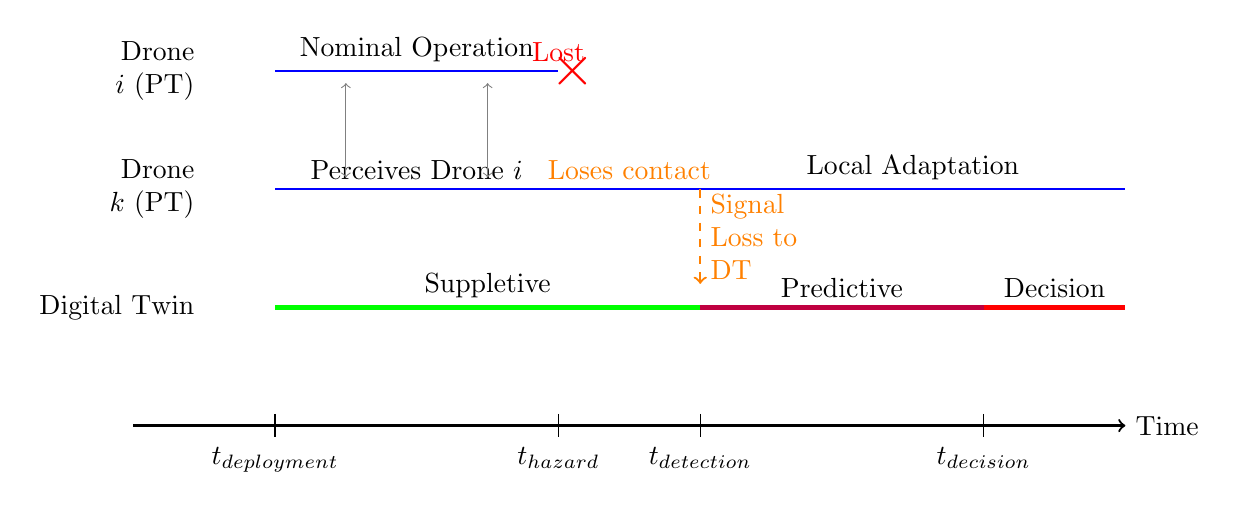
\begin{tikzpicture}[x=1.8cm, y=1.5cm]
    % Time axis
    \draw[->, thick] (0,0) -- (7,0) node[right] {Time};

    % Time markers
    \node[below] at (1,-0.1) {$t_{\text{deployment}}$};
    \draw (1,0.1) -- (1,-0.1);
    \node[below] at (3,-0.1) {$t_{\text{hazard}}$};
    \draw (3,0.1) -- (3,-0.1);
    \node[below, text width=1.5cm, align=center] at (4,-0.1) {$t_{\text{detection}}$};
    \draw (4,0.1) -- (4,-0.1);
    \node[below, text width=2cm, align=center] at (6,-0.1) {$t_{\text{decision}}$};
    \draw (6,0.1) -- (6,-0.1);

    % Drone i track (Lost)
    \node[left, text width=2cm, align=right] at (0.5, 3) {Drone $i$ (PT)};
    \draw[blue, thick] (1,3) -- (3,3);
    \node[above] at (2,3) {Nominal Operation};
    \node[red, xshift=5pt] at (3,3) {\huge $\times$};
    \node[above, red] at (3,3) {Lost};

    % Drone k track (Detects loss)
    \node[left, text width=2cm, align=right] at (0.5, 2) {Drone $k$ (PT)};
    \draw[blue, thick] (1,2) -- (7,2);
    \node[above] at (2,2) {Perceives Drone $i$};
    \draw[<->, gray] (1.5, 2.9) -- (1.5, 2.1);
    \draw[<->, gray] (2.5, 2.9) -- (2.5, 2.1);
    \node[above, orange] at (3.5,2) {Loses contact};
    \draw[->, orange, thick, dashed] (4, 2) -- (4, 1.2) node[midway, right, text width=1.5cm] {Signal Loss to DT};
    \node[above] at (5.5, 2) {Local Adaptation};

    % Digital Twin High-Level Phases
    \node[left, text width=2cm, align=right] at (0.5, 1) {Digital Twin};
    \draw[green, ultra thick] (1,1) -- (4,1);
    \node[above] at (2.5, 1) {Suppletive};
    \draw[purple, ultra thick] (4,1) -- (6,1);
    \node[above] at (5, 1) {Predictive};
    \draw[red, ultra thick] (6,1) -- (7,1);
    \node[above] at (6.5, 1) {Decision};

\end{tikzpicture}
\caption{High-level temporal sequence of PT/DT interaction. A hazard triggers detection by a PT drone, which sends an exception report to the DT. The DT transitions from a low-emission \emph{suppletive} state to an active \emph{predictive} state to analyze the situation, and then enters a \emph{decision} phase (e.g., spare injection, alert/strike recommendation).}
\label{fig:timeline_high_level}
\end{figure*}


\begin{figure*}[h!]
\centering
\begin{tikzpicture}[x=1.5cm, y=1.4cm]
  % Time axis
    \draw[->, thick] (0,0) -- (7,0);
    \node[right] at (7,0) {DT Simulation Time};

    % Time markers
    \node[below] at (1,-0.1) {$t_{\text{last\_known}}$};
    \draw (1,0.1) -- (1,-0.1);
    \node[below] at (3.5,-0.1) {$t_{\text{pre-hazard}}$};
    \draw (3.5,0.1) -- (3.5,-0.1);
    \node[below] at (4.5,-0.1) {$t_{\text{hazard}}$};
    \draw (4.5,0.1) -- (4.5,-0.1);
    \node[below, text width=2cm, align=center] at (5.5,-0.1) {$t_{\text{hazard}} + \Delta t$};
    \draw (5.5,0.1) -- (5.5,-0.1);

    % Main state line (conceptual)
    \node[left, text width=2.5cm, align=right] at (-0.5, 1) {DT Internal State};

    % Step 1: Restore State
    \draw[->, thick, brown, dotted] (4.4, 1) .. controls (3, 0.2) and (2, 0.2) .. (1.1, 1);
    \node[above, blue] at (2.5, 0) {(1) Restore State};

    % Step 2: Simulate Forward
    \draw[->, thick, blue, dashed] (1.1, 1) .. controls (2, 1.5) and (3, 1.5) .. (3.4, 1);
    \node[above, blue] at (2.25, 1.5) {(2) Simulate to Pre-Hazard};

    % Step 3: Interpolate
    \draw[->, thick, green!50!black, densely dotted] (3.4, 1) -- (4.7, 1);
    \node[above, green!50!black] at (3.9, 1.1) {(3) Interpolate};

    % Step 4: Update with Hazard
    \node[draw=red, fill=red!30, star, star points=5, star point ratio=2, minimum size=6pt] at (4.7, 1) {};
    \node[above, red, text width=2cm, align=center] at (4.5, 1.8) {(4) Update with Hazard};
    \draw[->, red, thick] (4.7, 1.8) -- (4.7, 1.1);

    % Step 5: Predict Future
    \draw[->, thick, purple] (4.6, 1) .. controls (5.5, 1.5) and (5.5, 1.5) .. (6, 1);
    \node[above, purple] at (5.75, 1.5) {(5) Predict Future};

  % Output to Decision Phase
  \draw[->, thick, black] (6, 1) -- (6.25, 1) node[text width=2cm,right] {Output to Decision Phase};

\end{tikzpicture}
\caption{Zoom into the DT's \emph{predictive} phase. Upon receiving an exception, the DT restores the last known state, synchronizes to the hazard time, and runs a what-if simulation to forecast outcomes and feed the downstream \emph{decision} phase.}
\label{fig:timeline_zoom}
\end{figure*}

\subsection{Complementary Roles}

\paragraph{Role Separation}
The hybrid architecture achieves layered resilience through role separation: PT distributed control provides immediate autonomous response to loss events, while DT monitoring validates whether self-adaptation suffices or spare deployment is required. Critically, the PT has no knowledge of the DT; each drone perceives itself as alone-in-the-world, and any support from the DT manifests only as the arrival of additional drones rather than explicit commands. This division enables furtive operation (minimal RF emissions) while maintaining strategic oversight through predictive simulation, and contributes to system antifragility \cite{Taleb2012Antifragile}.

\paragraph{Roles Impact}
In the hybrid PT/DT architecture, we adopt the following notation: $R_{0}$ denotes the trajectory immediately after the \emph{first attack}; $R_{1}$ denotes the trajectory after a \emph{second attack} under \emph{PT-only} self-adaptation (no DT intervention); and $R_{2}$ denotes the trajectory after the \emph{second attack} under \emph{PT+DT} with spare staging. Here $R$ refers to \emph{robustness} — the capacity to maintain function under hazards — not resilience (which typically quantifies the time during which hazards gain no impact). Let $Y$ denote the \emph{nominal} (pre-attack) coverage level. We distinguish two angles: $\alpha$ for the \emph{descent slope} immediately following an attack (steeper $\alpha$ indicates faster degradation) and $\beta$ for the \emph{recovery slope} (larger $\beta$ indicates faster restoration). Robustness obtains when the redundancy ratio $r \triangleq n_{\text{eff}}/P_{\text{total}}$ (equivalently per segment $\rho_i/L_i$) exceeds a mission threshold $r_{\min}$; when enough drones remain ($n_{\text{eff}} \ge n_{\min}$), PT’s distributed reorganization restores coverage and the recovery slope scales with $r$.

Three scenarios structure the robustness comparison (see Figures~\ref{fig:pt-only} and~\ref{fig:dt-plus-pt}):
\begin{itemize}
    \item \textbf{PT-only degradation relative to baseline} ($R_{1}$ vs $R_{0}$): after the second attack, PT-only follows the $R_{1}$ trajectory; with repeated hazards and fewer drones, robustness degrades relative to $R_{0}$. Metrics: $\alpha_{1} > \alpha_{0}$ (sharper descent), $\beta_{1} < \beta_{0}$ (slower recovery), $Y_{1} < Y_{0}$ (lower coverage floor), and $X_{1} > X_{0}$ (larger gaps). Overall: $R_{1} < R_{0}$.
    \item \textbf{PT+DT relative gain over PT-only} ($R_{2}$ vs $R_{1}$): after the second attack with spare staging, the system follows the $R_{2}$ trajectory, with improved outcomes relative to PT-only. Metrics: $\alpha_{2} \lesssim \alpha_{1}$ (equal or gentler descent due to rapid staging), $\beta_{2} > \beta_{1}$ (faster recovery), $Y_{2} > Y_{1}$ (higher coverage floor), and $X_{2} < X_{1}$ (smaller gaps). Overall: $R_{2} > R_{1}$.
    \item \textbf{PT+DT absolute performance vs baseline} ($R_{2}$ vs $R_{0}$): PT+DT targets recovery to baseline or better. Metrics: $\alpha_{2} \approx \alpha_{0}$ (comparable descent), $\beta_{2} \geq \beta_{0}$ (equal or faster recovery), $Y_{2} = Y$ (nominal coverage restored in both reset and antifragility cases), and $X_{2} \lesssim X_{0}$ (gaps controlled). Overall: $R_{2} \geq R_{0}$ (reset), or $R_{2} > R_{0}$ when spares abundant (antifragility).
\end{itemize}
The three-way comparison establishes that PT-only degrades under repeated attacks ($R_{1} < R_{0}$), PT+DT provides significant relative gain ($R_{2} > R_{1}$), and — critically — PT+DT preserves or exceeds first-attack performance ($R_{2} \geq R_{0}$), demonstrating not just relative advantage but absolute robustness restoration. Here, $R_{0}$ provides the common baseline for reference in both figures, while $R_{1}$ and $R_{2}$ contrast PT-only self-adaptation against PT+DT spare staging.

\subsubsection{Failure Detection and Resilience to Byzantine Events}

Silent drone failures are not possible within this architecture: neighbors continuously sense each other within radius $r_d$, and any silent disappearance is immediately detected by the affected drone's predecessor in the patrol circuit. Communication delay is similarly disambiguated: a physical loss triggers neighbor-based detection at the spatial level, whereas transient communication delays only affect when the loss is \emph{reported} to the DT. Only coordinated, near-simultaneous destruction of sufficient fleet segments can render a loss undetectable.

False positives (byzantine failures) occur when a drone incorrectly reports losing its predecessor—e.g., due to sensor noise or transient occlusion. The system exhibits graceful degradation:
\begin{itemize}
    \item \textbf{Immediate PT response}: The false-positive reporter accelerates to close the perceived gap and may overtake its predecessor. The predecessor, observing the unexpected overtake, raises an alarm and may trigger defensive signaling.
    \item \textbf{Over-triggered spare insertion}: The DT may dispatch an unnecessary spare based on the false loss. Local balancing absorbs the extra drone; density rebalancing grows stronger but does not destabilize the fleet.
    \item \textbf{Trade-off in reporting strategy}: Two design choices emerge: (a) \emph{Delayed sensing}: require persistent loss confirmation over multiple sensing cycles before notifying the DT, reducing false positives but lowering reactivity and furtivity; (b) \emph{Immediate notification with validation}: report immediately and let the DT cross-check via predictive simulation, accepting occasional false spare deployments. \textbf{The critical question is to calibrate this latency-fidelity trade-off} based on mission threat model and communication security constraints.
\end{itemize}

Beyond this immediate robustness comparison, the DT provides a \emph{dual temporal perspective} that fundamentally enhances decision quality. While PT operates on short-term reactive perception (local sensor data, immediate exceptions), the DT maintains both \emph{predictive} simulation (forward-looking trajectory projection) and \emph{historical} analysis (accumulated disruption patterns over mission duration). This historical view enables the DT to detect escalating threat intensity: for example, increasing frequency of PT exception alerts may signal intensified adversarial action, warranting preemptive spare staging or heightened monitoring thresholds even before individual attacks degrade coverage below mission-critical levels. The complementarity of short-term PT perception, forward-looking DT prediction, and backward-looking DT pattern recognition constitutes a multi-scale temporal awareness unavailable to either subsystem alone — a strategic advantage \emph{not implemented in the present work} but identified as a high-priority extension.

\begin{figure}[t]
    \centering
    % If file exists, include it; otherwise show a placeholder box
    \IfFileExists{figures/PT_only.png}{\includegraphics[width=\linewidth]{figures/PT_only.png}}{\fbox{\parbox{0.9\linewidth}{\centering Placeholder: figures/PT\_only.png}}}
    \caption{PT-only response (second attack) showing robustness degradation relative to first-attack baseline. Notation: $R_{0}$ = first attack trajectory (baseline); $R_{1}$ = second attack (PT only). Degradation metrics: $R_{1} < R_{0}$, $\alpha_{1} > \alpha_{0}$ (sharper descent), $\beta_{1} < \beta_{0}$ (slower recovery), $Y_{1} < Y_{0}$ (lower coverage floor), and $X_{1} > X_{0}$ (larger gaps).}
    \label{fig:pt-only}
\end{figure}

\begin{figure}[t]
    \centering
    % If file exists, include it; otherwise show a placeholder box
    \IfFileExists{figures/DT+PT.png}{\includegraphics[width=\linewidth]{figures/DT+PT.png}}{\fbox{\parbox{0.9\linewidth}{\centering Placeholder: figures/DT+PT.png}}}
    \caption{PT+DT response (second attack) with staged spares, demonstrating relative gain over PT-only and absolute performance restoration vs baseline. Notation: $R_{0}$ = first attack trajectory (baseline); $R_{1}$ = second attack (PT only); $R_{2}$ = second attack (PT+DT). Relative gain: $R_{2} > R_{1}$, $\alpha_{2} \lesssim \alpha_{1}$ (gentler descent), $\beta_{2} > \beta_{1}$ (faster recovery), $Y_{2} > Y_{1}$ (higher floor), and $X_{2} < X_{1}$ (smaller gaps). Absolute performance: $R_{2} \geq R_{0}$ (reset) or $R_{2} > R_{0}$ (antifragility when spares abundant).}
    \label{fig:dt-plus-pt}
\end{figure}

